\documentclass[12pt,a4paper]{article}

% --- Typography and Academic Standards ---
\usepackage[utf8]{inputenc}
\usepackage[T1]{fontenc}
\usepackage{mathptmx} % Times New Roman-like academic typography
\usepackage{geometry}
\geometry{margin=1in}
\usepackage{setspace}
\onehalfspacing
\usepackage{microtype}

% --- Tables, Graphics, and Formatting ---
\usepackage{booktabs}
\usepackage{tabularx}
\usepackage{longtable}
\usepackage{array}
\usepackage{graphicx}
\usepackage{caption}
\usepackage{subcaption}
\usepackage{float}
\usepackage{amsmath,amssymb}

% --- Code Listings (Strictly Monochrome) ---
\usepackage{listings}
\lstset{
    basicstyle=\ttfamily\footnotesize,
    breaklines=true,
    breakatwhitespace=true,
    frame=single,
    rulecolor=\color{black},
    numbers=left,
    numberstyle=\tiny\ttfamily,
    stepnumber=1,
    numbersep=8pt,
    showstringspaces=false,
    tabsize=2,
    captionpos=b,
    keywordstyle=\bfseries,
    commentstyle=\itshape,
    stringstyle=\ttfamily
}

% --- Hyperlinks (Strictly Monochrome - No Colored Boxes or Links) ---
\usepackage{hyperref}
\hypersetup{
    colorlinks=false,
    hidelinks,
    pdfborder={0 0 0},
    pdftitle={Research Rover: Installation, Configuration and Technical Documentation},
    pdfauthor={Akashdeep Singha},
    pdfsubject={Software Technical Documentation},
    pdfkeywords={Research Rover, Technical Documentation, FastAPI, React, Data Ingestion, Bibliometrics}
}

% --- Page Headers and Footers ---
\usepackage{fancyhdr}
\pagestyle{fancy}
\fancyhf{}
\fancyhead[R]{\textit{\nouppercase{\rightmark}}}
\fancyfoot[C]{\thepage}
\renewcommand{\headrulewidth}{0.4pt}
\renewcommand{\footrulewidth}{0.4pt}

% Section depth configuration
\setcounter{secnumdepth}{3}
\setcounter{tocdepth}{3}

\begin{document}

% ---------------------------------------------------------------------------
% TITLE PAGE
% ---------------------------------------------------------------------------
\begin{titlepage}
    \begin{center}
        \vspace*{0.5in}
        
        {\Large \textbf{TEZPUR UNIVERSITY}}\\[0.2cm]
        {\large Department of Computer Science and Engineering}\\[0.1cm]
        {\normalsize Napaam, Tezpur, Assam -- 784028, India}\\[1.5cm]
        
        \rule{\linewidth}{1.2pt}\\[0.4cm]
        {\huge \textbf{Research Rover: Installation, Configuration and Technical Documentation}}\\[0.3cm]
        {\large \textbf{An Intelligent Research Discovery, Bibliometric Analysis, and Universal Ingestion Platform}}\\[0.2cm]
        \rule{\linewidth}{1.2pt}\\[2.0cm]
        
        \begin{minipage}{0.85\textwidth}
            \begin{tabular}{ll}
                \textbf{Project Name:} & Research Rover \\
                \textbf{Prepared By:} & Akashdeep Singha \\
                \textbf{Programme:} & M.Tech in Data Science \\
                \textbf{Department:} & Computer Science and Engineering \\
                \textbf{Institution:} & Tezpur University \\
                \textbf{Documentation Version:} & 1.0 \\
                \textbf{Date of Documentation:} & 17 November 2026 \\
                \textbf{Repository URL:} & \url{https://github.com/Akashdeep4565/Research_Rover} \\
            \end{tabular}
        \end{minipage}
        
        \vfill
        
        {\normalsize A Formal Academic Software Engineering Technical Reference\\Prepared for Project Review and Developer Onboarding}
        
        \vspace*{0.5in}
    \end{center}
\end{titlepage}

% ---------------------------------------------------------------------------
% TABLE OF CONTENTS & LISTS
% ---------------------------------------------------------------------------
\newpage
\pagenumbering{roman}
\tableofcontents
\newpage
\listoffigures
\vspace{1cm}
\listoftables
\newpage
\pagenumbering{arabic}
\setcounter{page}{1}

% ---------------------------------------------------------------------------
% SECTIONS
% ---------------------------------------------------------------------------
\section{Introduction}
\label{sec:introduction}

\subsection{Overview of Research Rover}
\textbf{Research Rover} is a modern, full-stack, artificial intelligence-assisted research discovery, bibliometric analytics, and literature synthesis platform. Developed to address the escalating complexity of scientific literature exploration, the platform bridges the gap between multi-source bibliographic retrieval, high-dimensional textual analytics, dense vector semantic search, and interactive conversational artificial intelligence.

In contemporary data science and academic research, scholars routinely navigate thousands of published manuscripts across fragmented repositories. Research Rover establishes a consolidated operational workflow wherein users can query biomedical and multidisciplinary digital libraries, extract rich metadata, visualize keyword associations and international research networks, generate dense semantic representations, and interrogate document corpora via retrieval-augmented generation (RAG).

\subsection{Purpose and Core Capabilities}
The primary objective of Research Rover is to provide an end-to-end analytical pipeline that minimizes the friction between literature collection and thematic knowledge synthesis. The platform delivers seven primary capabilities:

\begin{enumerate}
    \item \textbf{Intelligent Multi-Source Paper Discovery:} Federated retrieval interfacing with the National Center for Biotechnology Information (NCBI) PubMed database via E-utilities \cite{sayers2022eutilities} and the OpenAlex scholarly catalog \cite{priem2022openalex}, featuring automated abbreviation expansion, typographical error correction, and neural semantic re-ranking via MedCPT \cite{jin2023medcpt}.
    \item \textbf{Automated Full-Text Extraction:} Robust web scraping utilizing Crawl4AI and BeautifulSoup4 to extract full-text manuscript content from publisher digital object identifier (DOI) landing pages, with graceful fallback to comprehensive abstract content.
    \item \textbf{Dense Vector Semantic Search:} High-performance vector indexing using the 768-dimensional Sentence Transformers model (\texttt{all-mpnet-base-v2}) \cite{reimers2019sentence} coupled with Facebook AI Similarity Search (FAISS) \cite{johnson2019billion} for sub-millisecond context retrieval.
    \item \textbf{Conversational Research Synthesis:} An intelligent retrieval-augmented generation (RAG) assistant powered by Google Gemini (\texttt{gemini-2.5-flash}) supporting query decomposition, context deduplication, and verifiable manuscript citations.
    \item \textbf{Bibliometric Network Analytics:} Quantitative text mining modules calculating keyword frequency distributions, co-occurrence presence matrices, and interactive two-dimensional and three-dimensional international co-authorship collaboration graphs.
    \item \textbf{Universal Dataset Ingestion and Normalization:} An intelligent data processing layer that standardizes heterogeneous research-paper CSV files from arbitrary academic databases into a 20-field canonical schema.
    \item \textbf{Dataset Quality and Feature Readiness Evaluation:} An automated assessment engine computing multi-attribute quality scores (0--100) and deterministically evaluating system readiness across seven analytical features.
\end{enumerate}

\subsection{Intended Audience}
Research Rover is designed for postgraduate researchers, academic faculty, data scientists, research laboratory teams, and literature review specialists. The technical documentation presented herein is intended for software engineers, systems administrators, and academic developers tasked with downloading, configuring, deploying, maintaining, or extending the Research Rover codebase.

\subsection{Technology Stack Summary}
The application employs a decoupled client-server architecture built upon modern web and data engineering technologies:

\begin{itemize}
    \item \textbf{Backend Core:} Python 3.11+ asynchronous runtime; FastAPI \cite{fastapi2020} for high-performance RESTful APIs; Uvicorn Asynchronous Server Gateway Interface (ASGI); Pydantic v2 for data validation and schema serialization.
    \item \textbf{Machine Learning \& NLP:} PyTorch, Hugging Face Transformers, Sentence Transformers (\texttt{all-mpnet-base-v2}), MedCPT Query/Article Encoders (\texttt{ncbi/MedCPT-Query-Encoder}, \texttt{ncbi/MedCPT-Article-Encoder}), and FAISS-CPU for dense vector clustering and nearest-neighbor search.
    \item \textbf{Frontend User Interface:} React 19 single-page application (SPA); Vite 6 build engine; TypeScript 5.7; Tailwind CSS 3.4 for utility-first responsive styling; Radix UI primitives; Framer Motion 12 for transition dynamics; Three.js and React Force Graph (2D/3D) for network graph visualization.
    \item \textbf{Data Ingestion \& Storage:} Pandas and NumPy for tabular data operations; JSON metadata sidecars; disk-persisted CSV files and serialized FAISS vector indexes.
\end{itemize}

\newpage
\section{System Requirements}
\label{sec:requirements}

\subsection{Hardware and Operational Requirements}
To ensure reliable operation of the backend language models, embedding pipelines, and responsive frontend rendering, the host environment must meet the verified hardware specifications detailed below.

\begin{itemize}
    \item \textbf{Processor (CPU):} Minimum 4 physical cores (x86\_64 architecture). AVX2 instruction set support is strongly recommended for optimized FAISS vector similarity operations and PyTorch tensor calculations.
    \item \textbf{System Memory (RAM):}
    \begin{itemize}
        \item \textit{Minimum:} 8 GB RAM (sufficient for core API services and basic dataset ingestion).
        \item \textit{Recommended:} 16 GB RAM (necessary when loading Sentence Transformers and MedCPT neural re-ranking models into memory concurrently).
    \end{itemize}
    \item \textbf{Disk Storage:} Minimum 5 GB free disk space. This accommodates the Python virtual environment, Node.js modules, local cache directories for Hugging Face transformer models (\texttt{\textasciitilde/.cache/huggingface}), temporary web scraping artifacts, and exported bibliographic datasets.
    \item \textbf{Network Connectivity:} Persistent broadband internet connection is required for initial model weight downloads, package installations, and live querying of the NCBI PubMed and Google Gemini APIs.
\end{itemize}

\subsection{Operating System and Software Dependencies}
Research Rover is cross-platform and operates on:
\begin{itemize}
    \item \textbf{Windows:} Windows 10 or Windows 11 (64-bit) with PowerShell 5.1 or PowerShell 7+.
    \item \textbf{Linux:} Ubuntu 20.04 LTS or later, Debian 11+, or Fedora 36+ (64-bit).
    \item \textbf{macOS:} macOS 12.0 (Monterey) or later (Apple Silicon or Intel x86\_64).
\end{itemize}

The foundational software environments must be pre-installed on the host system:
\begin{enumerate}
    \item \textbf{Python Runtime:} Python 3.11.x (verified 3.11.0 to 3.12.x). A 64-bit installation is strictly mandatory; 32-bit Python runtimes cannot allocate sufficient address space for PyTorch and FAISS.
    \item \textbf{Node.js Runtime:} Node.js version 18.x LTS, 20.x LTS, or 22.x LTS.
    \item \textbf{Package Managers:} \texttt{pip} (Python package installer) version 23.0+ and \texttt{npm} (Node package manager) version 9.0+.
    \item \textbf{Version Control:} Git version 2.30+ for repository cloning and revision tracking.
\end{enumerate}

\subsection{API Credentials and Configuration Keys}
Table~\ref{tab:requirements_summary} distinguishes between mandatory and optional software and credential requirements.

\begin{table}[H]
\centering
\caption{System Requirements and External Dependency Classification}
\label{tab:requirements_summary}
\begin{tabularx}{\textwidth}{l p{3.2cm} X l}
\toprule
\textbf{Component} & \textbf{Requirement} & \textbf{Operational Function} & \textbf{Status} \\
\midrule
Python 3.11+ & Runtime Environment & Executes FastAPI backend and AI pipelines & Mandatory \\
Node.js 18+ / npm & Runtime Environment & Compiles and runs Vite / React frontend & Mandatory \\
Git & Version Control & Clones and updates repository source tree & Mandatory \\
Google Gemini API Key & \texttt{GOOGLE\_GENAI\_API\_KEY} & Powers conversational AI assistant and RAG & Mandatory \\
User Contact Email & \texttt{EMAIL} & Transmitted in NCBI E-utilities API headers & Mandatory \\
PubMed API Key & \texttt{PUBMED\_API\_KEY} & Increases NCBI rate limits from 3 to 10 req/s & Optional \\
OpenAlex API Key & \texttt{OPENALEX\_API\_KEY} & Raises OpenAlex rate limits and priority & Optional \\
FAISS CPU Index & Disk Storage & Enables dense vector semantic search & Feature-Specific \\
\bottomrule
\end{tabularx}
\end{table}

\noindent \textbf{Security Notice:} API keys and secrets must never be committed to source code repositories. Research Rover utilizes local \texttt{.env} configuration files excluded from version control via \texttt{.gitignore}.

\newpage
\section{Downloading and Installation}
\label{sec:installation}

\subsection{Downloading Research Rover from GitHub}
The complete Research Rover source code is maintained on GitHub. Developers can obtain the project using Git or by downloading an archive.

\subsubsection{Method A: Cloning via Git (Recommended)}
Open Windows PowerShell, macOS Terminal, or Linux Bash, navigate to your target workspace directory, and execute:

\begin{lstlisting}[language=bash, caption={Cloning Research Rover from GitHub}]
git clone https://github.com/Akashdeep4565/Research_Rover.git
cd Research_Rover
\end{lstlisting}

\subsubsection{Method B: Downloading Archive (ZIP Alternative)}
If Git is not installed on the host machine:
\begin{enumerate}
    \item Navigate to the official repository URL: \url{https://github.com/Akashdeep4565/Research_Rover}.
    \item Click the \textbf{Code} button and select \textbf{Download ZIP}.
    \item Extract the downloaded \texttt{Research\_Rover-main.zip} archive to the local directory (e.g., \texttt{E:\textbackslash Research\_Rover}).
    \item Open a terminal window and navigate into the extracted root directory.
\end{enumerate}

\begin{figure}[H]
\centering
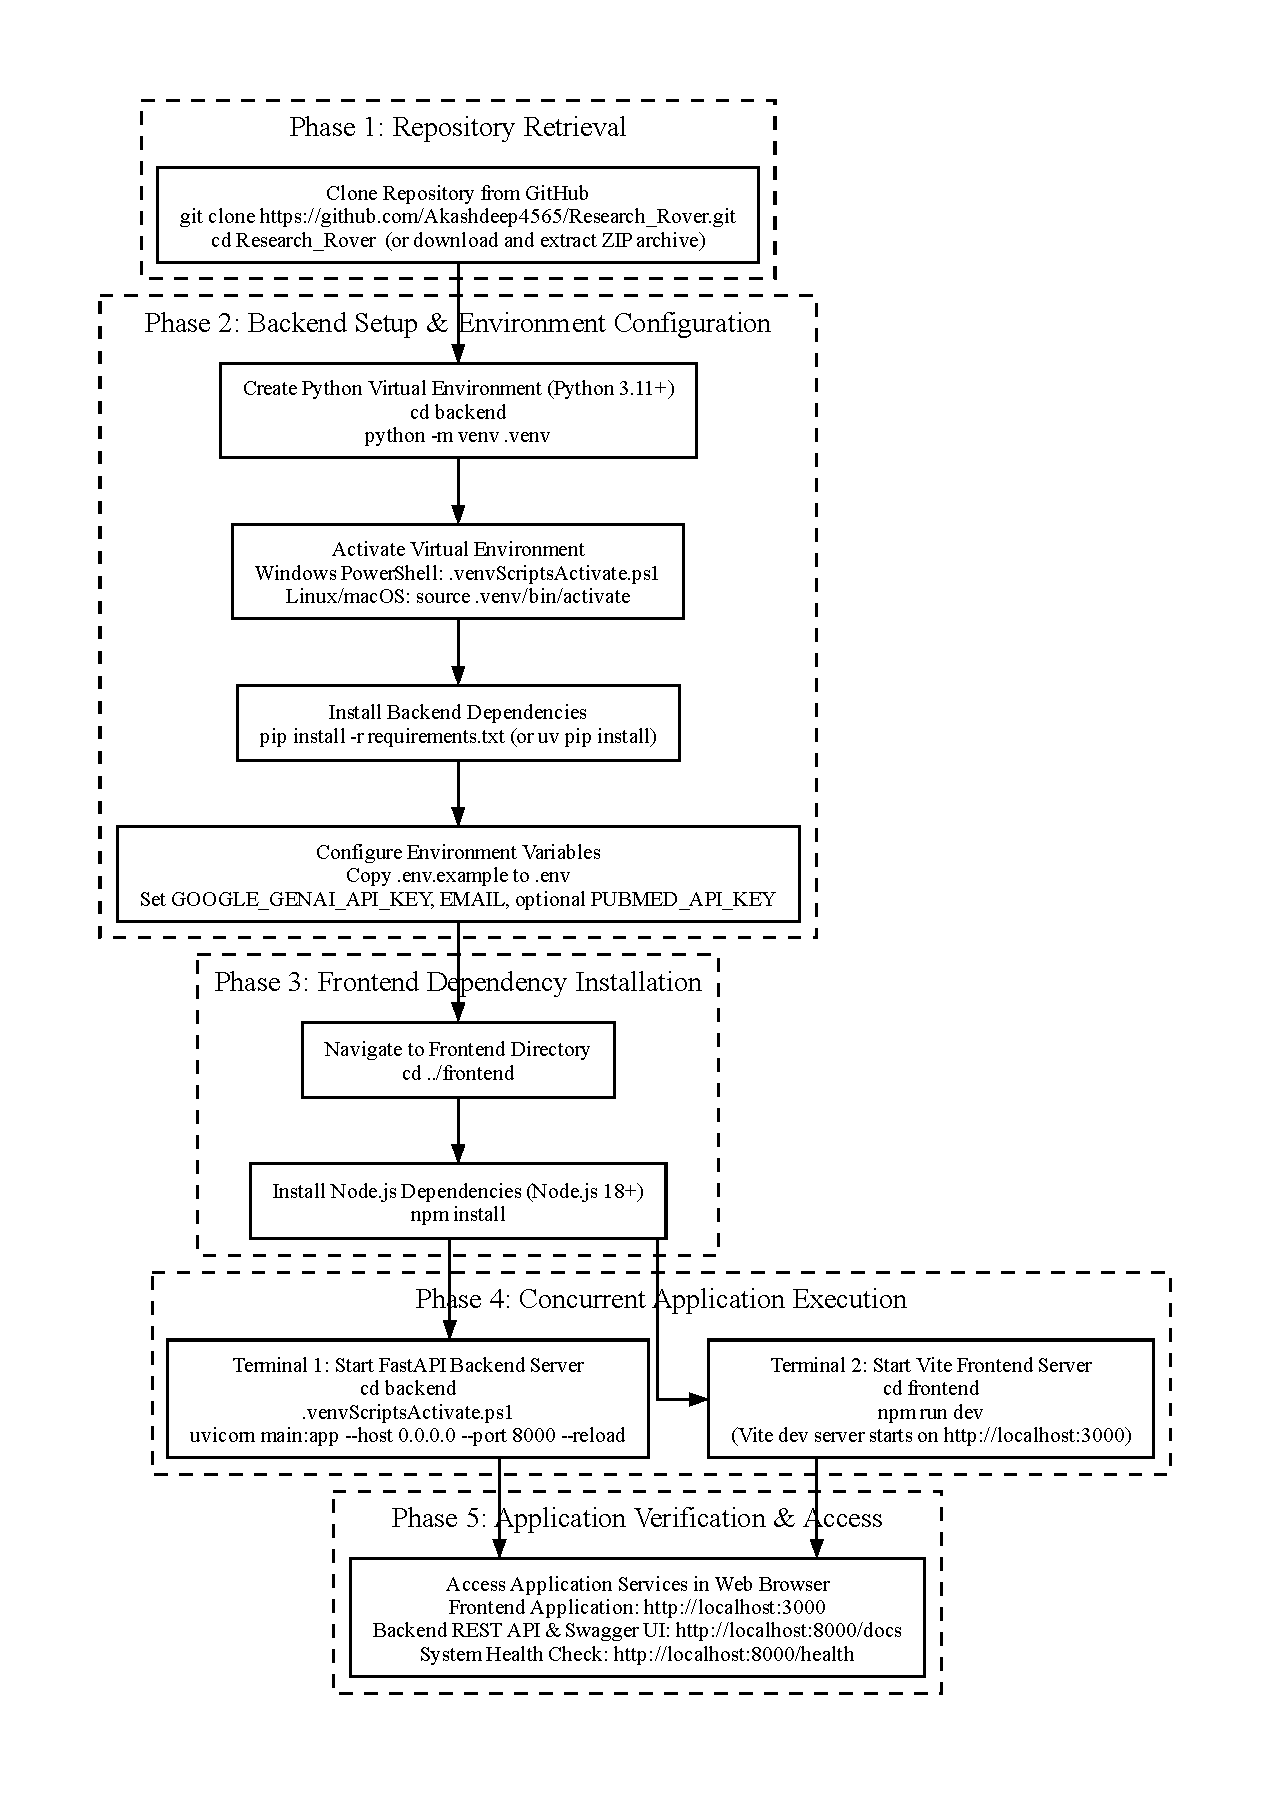
\includegraphics[width=0.88\textwidth]{figures/installation_workflow.pdf}
\caption{End-to-End Installation, Configuration, and Execution Workflow}
\label{fig:installation_workflow}
\end{figure}

Figure~\ref{fig:installation_workflow} illustrates the end-to-end procedural workflow required to set up both backend and frontend environments.

\subsection{Backend Installation and Environment Setup}
The backend application is encapsulated within the \texttt{backend/} directory. All dependency installations should be isolated within a dedicated Python virtual environment.

\subsubsection{Step 1: Create and Activate Python Virtual Environment}
Navigate to the \texttt{backend} subdirectory:

\begin{lstlisting}[language=bash, caption={Creating and Activating Virtual Environment}]
# Navigate to backend directory
cd backend

# Create isolated virtual environment named .venv
python -m venv .venv

# Activate on Windows PowerShell:
.venv\Scripts\Activate.ps1

# Activate on Windows Command Prompt (cmd.exe):
.venv\Scripts\activate.bat

# Activate on macOS / Linux:
source .venv/bin/activate
\end{lstlisting}

\noindent \textit{PowerShell Execution Policy Note:} If Windows PowerShell returns a script execution policy error (\texttt{PSSecurityException}), permit local script execution by running:
\begin{lstlisting}[language=powershell]
Set-ExecutionPolicy -ExecutionPolicy RemoteSigned -Scope CurrentUser
\end{lstlisting}

\subsubsection{Step 2: Install Backend Python Dependencies}
Ensure \texttt{pip} is upgraded to the latest version, then install all pinned dependencies from \texttt{requirements.txt}:

\begin{lstlisting}[language=bash, caption={Installing Backend Python Packages}]
python -m pip install --upgrade pip
pip install -r requirements.txt
\end{lstlisting}

\noindent The installation encompasses key packages including \texttt{fastapi==0.115.6}, \texttt{uvicorn==0.34.0}, \texttt{torch==2.7.0}, \texttt{transformers==4.52.2}, \texttt{sentence-transformers==4.1.0}, \texttt{faiss-cpu==1.11.0}, \texttt{google-generativeai==0.8.5}, \texttt{Crawl4AI==0.6.3}, and \texttt{pandas==2.2.3}.

\subsubsection{Step 3: Configure Backend Environment Variables}
The backend relies on environment variables defined in a \texttt{.env} file located at \texttt{backend/.env}. A reference template is provided in \texttt{backend/.env.example}. Copy the template:

\begin{lstlisting}[language=bash, caption={Initializing Environment Configuration}]
# On Windows PowerShell:
Copy-Item .env.example .env

# On macOS / Linux:
cp .env.example .env
\end{lstlisting}

Open \texttt{backend/.env} in a text editor and populate the verified configuration values:

\begin{lstlisting}[caption={Example backend/.env Configuration File}]
# Mandatory: Google Gemini API Key for Chat & RAG
GOOGLE_GENAI_API_KEY="AIzaSyYourActualGeminiApiKeyGoesHere"

# Mandatory: Valid email address for NCBI PubMed API etiquette
EMAIL="researcher@university.edu"

# Optional: Personal NCBI PubMed API Key (increases rate limit to 10 req/s)
PUBMED_API_KEY=""

# Optional: OpenAlex API key for high-throughput scholarly search
OPENALEX_API_KEY=""
\end{lstlisting}

\subsection{Frontend Installation and Setup}
The frontend user interface is contained in the \texttt{frontend/} directory and is managed via Node.js and npm.

\subsubsection{Step 1: Navigate and Install Node Dependencies}
Open a new terminal window or navigate out of the backend directory into \texttt{frontend}:

\begin{lstlisting}[language=bash, caption={Installing Frontend Dependencies}]
cd ../frontend
npm install
\end{lstlisting}

\noindent This installs all packages specified in \texttt{package.json}, including React 19, Vite 6, Tailwind CSS, Lucide icons, Three.js, and Radix UI components.

\subsubsection{Step 2: Verify Vite Development Server Configuration}
The frontend development server configuration is defined in \texttt{frontend/vite.config.ts}:

\begin{lstlisting}[language=javascript, caption={Vite Server Port and Reverse Proxy in vite.config.ts}]
export default defineConfig({
  plugins: [react()],
  resolve: {
    alias: {
      "@": path.resolve(__dirname, "./src"),
    },
  },
  server: {
    port: 3000,
    proxy: {
      '/api': {
        target: 'http://localhost:8000',
        changeOrigin: true,
      },
    },
  },
})
\end{lstlisting}

\noindent As configured, the Vite dev server binds to port \textbf{3000} and automatically proxies all API requests beginning with \texttt{/api} to the FastAPI backend running on \texttt{http://localhost:8000}.

\newpage
\section{Running the Application}
\label{sec:execution}

\subsection{The Two-Terminal Execution Model}
Research Rover operates as an asynchronous decoupled architecture. The backend API server and the frontend client interface must run concurrently in two separate terminal sessions.

\begin{figure}[H]
\centering
\begin{minipage}{0.48\textwidth}
\textbf{Terminal 1: FastAPI Backend}
\begin{lstlisting}[language=bash]
cd E:\Research_Rover\backend
.venv\Scripts\Activate.ps1
uvicorn main:app --host 0.0.0.0 --port 8000 --reload
\end{lstlisting}
\end{minipage}
\hfill
\begin{minipage}{0.48\textwidth}
\textbf{Terminal 2: Vite Frontend}
\begin{lstlisting}[language=bash]
cd E:\Research_Rover\frontend
npm run dev
\end{lstlisting}
\end{minipage}
\caption{Two-Terminal Execution Commands for Running Research Rover Locally}
\label{fig:two_terminal_box}
\end{figure}

\subsection{Starting the Services}

\subsubsection{Terminal 1: Start the Backend Server}
In your first terminal, activate the Python virtual environment and launch Uvicorn:

\begin{lstlisting}[language=bash, caption={Launching FastAPI Backend Server}]
cd E:\Research_Rover\backend
.venv\Scripts\Activate.ps1
uvicorn main:app --host 0.0.0.0 --port 8000 --reload
\end{lstlisting}

\noindent Upon successful startup, the terminal logs will display:
\begin{lstlisting}
INFO:     Started server process [pid]
INFO:     Waiting for application startup.
INFO:     Starting Research Rover API...
INFO:     Research Rover API started successfully
INFO:     Uvicorn running on http://0.0.0.0:8000 (Press CTRL+C to quit)
\end{lstlisting}

\noindent The application lifespan context manager initializes the data directory at \texttt{E:\textbackslash Research\_Rover\textbackslash data} and begins asynchronous background warm-up of transformer models without blocking incoming HTTP traffic.

\subsubsection{Terminal 2: Start the Frontend Development Server}
In your second terminal, navigate to the frontend directory and start Vite:

\begin{lstlisting}[language=bash, caption={Launching Vite Frontend Server}]
cd E:\Research_Rover\frontend
npm run dev
\end{lstlisting}

\noindent The console output will confirm:
\begin{lstlisting}
  VITE v6.2.0  ready in 480 ms

  ➜  Local:   http://localhost:3000/
  ➜  Network: use --host to expose
  ➜  press h + enter to show help
\end{lstlisting}

\subsection{Application Access URLs and Health Verification}
Once both servers are operational, access the application and documentation interfaces via any standard web browser using the URLs listed in Table~\ref{tab:access_urls}.

\begin{table}[H]
\centering
\caption{Research Rover Local Access URLs and Service Interfaces}
\label{tab:access_urls}
\begin{tabularx}{\textwidth}{l X l}
\toprule
\textbf{Interface} & \textbf{Network URL} & \textbf{Primary Purpose} \\
\midrule
Web Application UI & \url{http://localhost:3000} & Interactive research portal and dashboards \\
Backend API Base & \url{http://localhost:8000} & Core REST API service \\
OpenAPI Swagger UI & \url{http://localhost:8000/docs} & Interactive API testing and parameter explorer \\
ReDoc Documentation & \url{http://localhost:8000/redoc} & Formal REST API specification documentation \\
System Health Check & \url{http://localhost:8000/health} & Real-time model and runtime status telemetry \\
Root Ping Endpoint & \url{http://localhost:8000/} & Lightweight health check (\texttt{\{"status": "healthy"\}}) \\
\bottomrule
\end{tabularx}
\end{table}

\subsection{Terminating the Application}
To shut down the platform cleanly:
\begin{enumerate}
    \item Focus on Terminal 2 (Frontend) and press \texttt{Ctrl + C}. Confirm termination if prompted.
    \item Focus on Terminal 1 (Backend) and press \texttt{Ctrl + C}. Uvicorn will execute the lifespan shutdown sequence and release bound network ports.
\end{enumerate}

\newpage
\section{Overall System Architecture}
\label{sec:architecture}

\subsection{Architectural Paradigm}
Research Rover is designed following a modular, five-tier layered software architecture. The platform enforces strict separation of concerns, decoupling user presentation, API dispatching, scientific domain computation, local persistence, and external data provider communications.

\begin{figure}[H]
\centering
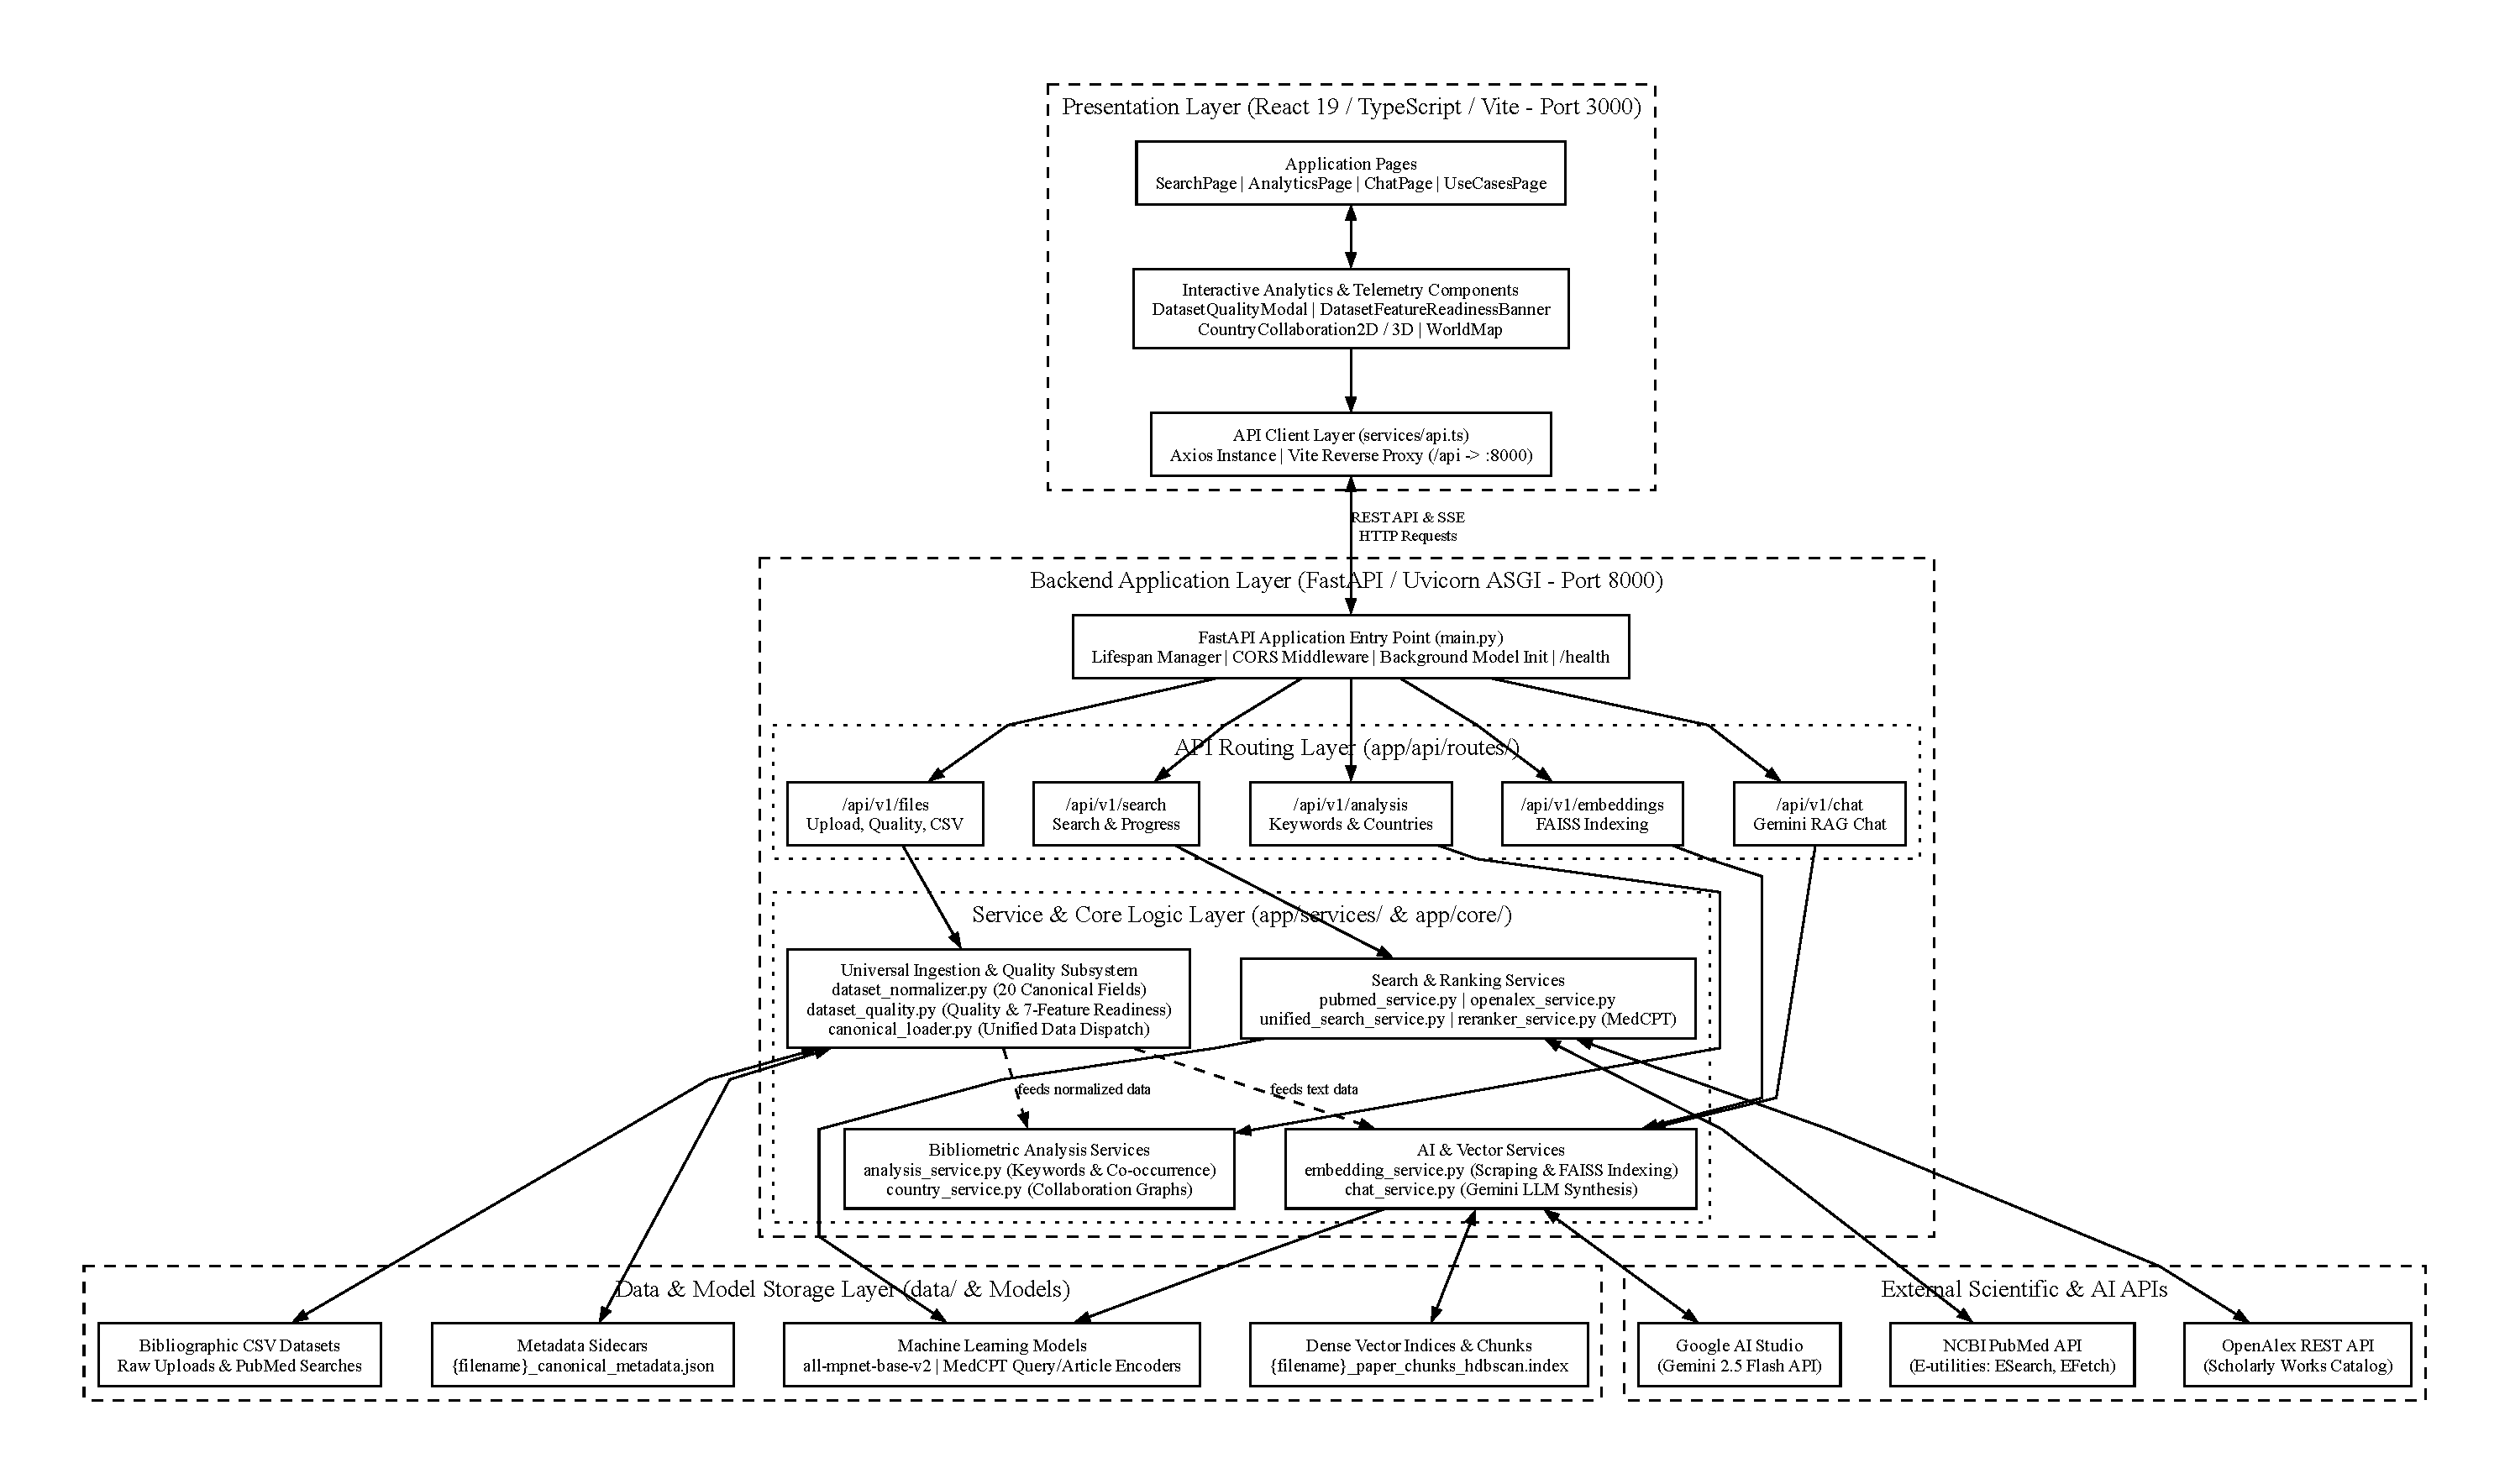
\includegraphics[width=0.95\textwidth]{figures/system_architecture.pdf}
\caption{Overall Multi-Tier System Architecture of Research Rover}
\label{fig:system_architecture}
\end{figure}

As depicted in Figure~\ref{fig:system_architecture}, the system consists of five cohesive layers:

\subsection{Detailed Architectural Layers}

\subsubsection{1. Presentation Layer (Frontend SPA)}
The presentation tier is implemented as a client-side Single-Page Application (SPA) utilizing React 19 and TypeScript. It includes:
\begin{itemize}
    \item \textbf{Routing and View Pages:} Managed by React Router v7, presenting the Search Portal (\texttt{SearchPage.tsx}), Bibliometric Analytics Dashboard (\texttt{AnalyticsPage.tsx}), Conversational RAG Interface (\texttt{ChatPage.tsx}), and Project Use-Case Demonstrations (\texttt{UseCasesPage.tsx}).
    \item \textbf{Diagnostic Components:} Including the \texttt{DatasetQualityModal.tsx} for inspecting uploaded dataset health, and \texttt{DatasetFeatureReadinessBanner.tsx} for informing users of analytical feature readiness.
    \item \textbf{Visualisation Engines:} Integrating Three.js and ForceGraph for dynamic two-dimensional and three-dimensional international research collaboration topologies.
    \item \textbf{API Client Module:} Encapsulated within \texttt{frontend/src/services/api.ts}, utilizing Axios with request timeouts and automatic payload transformation.
\end{itemize}

\subsubsection{2. API Dispatch and Routing Layer (FastAPI Backend)}
The entry point of the server application is \texttt{backend/main.py}, operating under the Uvicorn ASGI server. This layer manages:
\begin{itemize}
    \item \textbf{Cross-Origin Resource Sharing (CORS):} Configured via FastAPI \texttt{CORSMiddleware} to allow seamless communication between the frontend client and backend API.
    \item \textbf{Modular Route Controllers:} Subdividing incoming requests across six route controllers: \texttt{search.py}, \texttt{files.py}, \texttt{analysis.py}, \texttt{embeddings.py}, \texttt{chat.py}, and \texttt{system.py}.
    \item \textbf{Lifespan Task Execution:} Managing background thread pools for non-blocking model pre-loading.
\end{itemize}

\subsubsection{3. Business Logic and Service Layer}
This layer houses the analytical, retrieval, and machine learning logic:
\begin{itemize}
    \item \textbf{Search Subsystem:} Dispatches queries to PubMed and OpenAlex, standardizes responses, and applies MedCPT zero-shot bi-encoder re-ranking.
    \item \textbf{Universal Ingestion Subsystem:} Executes four-tier header matching, data cleaning, multi-attribute quality scoring, and seven-feature readiness verification.
    \item \textbf{Bibliometric Analytics Subsystem:} Extracts author country affiliations, builds co-occurrence networks, and calculates keyword frequency matrices.
    \item \textbf{Vector and AI Subsystem:} Chunks texts, computes 768-dimensional embeddings via Sentence Transformers, indexes vectors using FAISS, and synthesizes answers via Google Gemini.
\end{itemize}

\subsubsection{4. Persistence and Storage Layer}
All persistent data is organized within the root \texttt{data/} directory:
\begin{itemize}
    \item \textbf{Tabular Datasets:} Raw and normalized research paper CSV files.
    \item \textbf{Metadata Sidecars:} Dedicated \texttt{*\_canonical\_metadata.json} sidecar files storing quality scores, field mappings, and feature readiness telemetry.
    \item \textbf{Vector Indexes:} FAISS binary indexes (\texttt{*\_paper\_chunks\_hdbscan.index}) and associated chunk mapping files.
    \item \textbf{Full-Text Cache:} JSON mappings correlating paper DOIs with scraped full-text content.
\end{itemize}

\subsubsection{5. External Research and Intelligence Providers}
Research Rover interfaces securely with external academic and computational services:
\begin{itemize}
    \item \textbf{NCBI E-utilities API:} Provides access to over 35 million biomedical citations via \texttt{esearch.fcgi} and \texttt{efetch.fcgi}.
    \item \textbf{OpenAlex REST API:} Provides multidisciplinary scholarly graph data across global institutions.
    \item \textbf{Google AI Studio (Gemini 2.5 Flash):} Powers advanced natural language understanding and context synthesis.
\end{itemize}

\newpage
\section{Main Application Modules}
\label{sec:modules}

\subsection{Module Inventory and Source Code Organization}
The backend architecture is structured around ten core operational modules located across \texttt{backend/app/services/}, \texttt{backend/app/api/routes/}, and \texttt{backend/features/}. 

\begin{figure}[H]
\centering
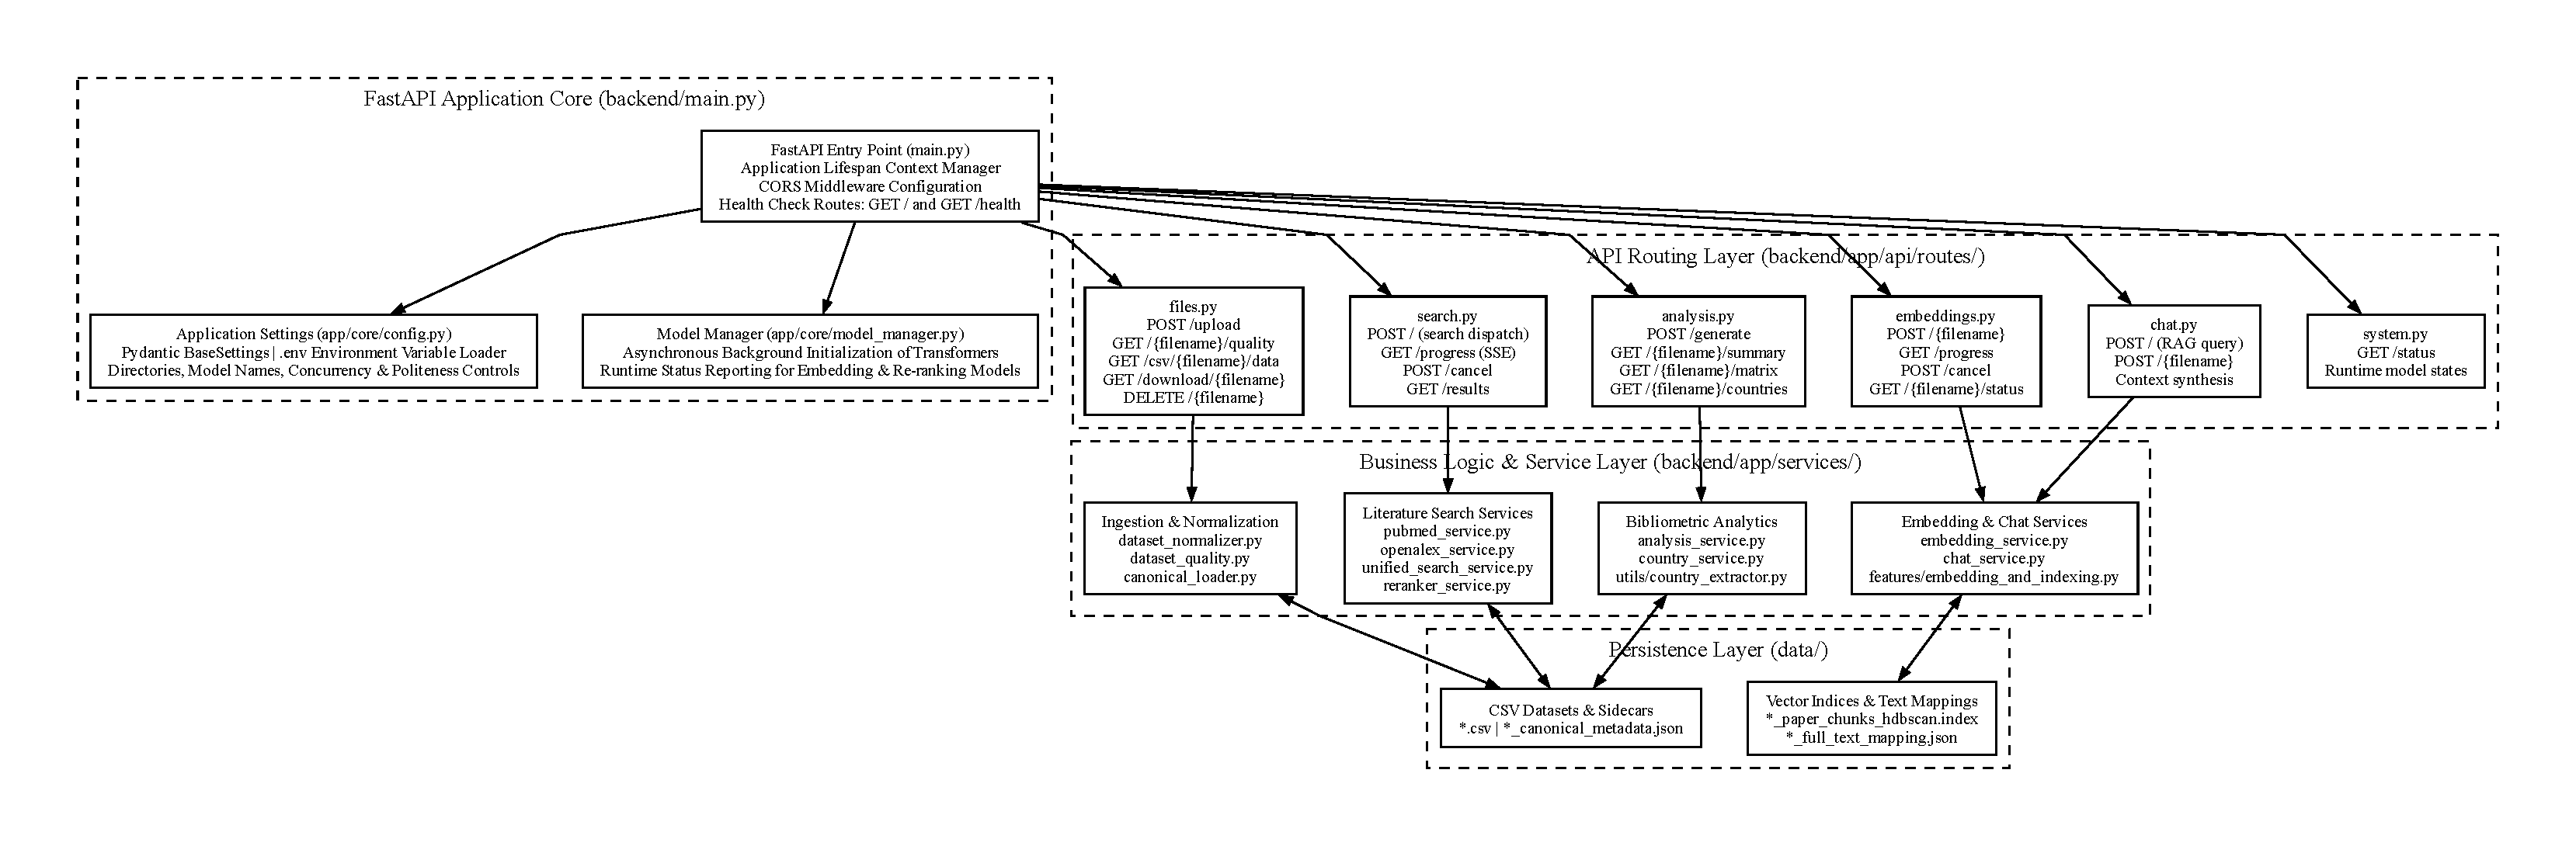
\includegraphics[width=0.92\textwidth]{figures/backend_architecture.pdf}
\caption{Detailed Internal Architecture and Subsystem Interactions of the Backend}
\label{fig:backend_architecture}
\end{figure}

Figure~\ref{fig:backend_architecture} illustrates the routing, service orchestration, and data access flow within the backend.

\subsection{Detailed Technical Description of Modules}

\subsubsection{1. Research Paper Search Module}
\textbf{Files:} \texttt{app/services/search\_service.py}, \texttt{app/api/routes/search.py}\\
Coordinates literature retrieval requests. Supports asynchronous job execution, real-time stage progress reporting via Server-Sent Events (SSE), query cancellation, and export of search results to timestamped CSV files.

\subsubsection{2. PubMed Integration Module}
\textbf{Files:} \texttt{app/services/pubmed\_service.py}, \texttt{app/services/pubmed\_affiliation\_enricher.py}\\
Interfaces directly with NCBI E-utilities. Performs query translation, abbreviation expansion, XML response parsing, author list parsing, MeSH term extraction, and affiliation country resolution.

\subsubsection{3. OpenAlex Integration Module}
\textbf{Files:} \texttt{app/services/openalex\_service.py}\\
Queries the OpenAlex API to fetch multidisciplinary scholarly literature. Handles pagination, DOI normalization, citation counts, concept tags, and institutional affiliation mapping.

\subsubsection{4. Unified Search and Re-ranking Module}
\textbf{Files:} \texttt{app/services/unified\_search\_service.py}, \texttt{app/services/reranker_service.py}\\
Enables simultaneous federated querying across PubMed and OpenAlex with result deduplication based on normalized DOIs. Incorporates NCBI's MedCPT bi-encoder models (\texttt{MedCPT-Query-Encoder} and \texttt{MedCPT-Article-Encoder}) to re-score candidate manuscripts against the search query, placing semantically relevant papers at the top of the result list.

\subsubsection{5. Keyword Analysis Module}
\textbf{Files:} \texttt{app/services/analysis\_service.py}, \texttt{app/api/routes/analysis.py}\\
Performs natural language tokenization, lemmatization, and stop-word filtering across research titles, abstracts, and author keywords. Computes term frequency distributions and outputs \texttt{*\_analysis\_keyword\_frequency.csv}.

\subsubsection{6. Keyword Co-occurrence Analysis Module}
\textbf{Files:} \texttt{app/services/analysis\_service.py}\\
Constructs symmetric co-occurrence presence matrices measuring the pairwise frequency with which research concepts appear within the same manuscript. Generates \texttt{*\_analysis\_keyword\_presence\_matrix.csv} for cluster analysis and thematic mapping.

\subsubsection{7. Country Collaboration Analysis Module}
\textbf{Files:} \texttt{app/services/country\_service.py}, \texttt{app/utils/country\_extractor.py}\\
Parses author affiliation text strings using regular expressions and international country dictionaries. Builds undirected collaboration network graphs where nodes represent sovereign nations and edge weights quantify co-authored publications. Produces telemetry for interactive 2D and 3D globe visualizations.

\subsubsection{8. AI Research Assistant (RAG) Module}
\textbf{Files:} \texttt{app/services/chat\_service.py}, \texttt{app/api/routes/chat.py}\\
Implements an advanced Retrieval-Augmented Generation (RAG) conversational pipeline. Complex user queries are decomposed into targeted sub-queries, evaluated against the FAISS dense vector store, deduplicated, and formatted into an evidence context passed to Google Gemini (\texttt{gemini-2.5-flash}) with instructions to generate cited answers.

\subsubsection{9. Embedding and Vector Indexing Module}
\textbf{Files:} \texttt{app/services/embedding\_service.py}, \texttt{features/embedding\_and\_indexing.py}\\
Manages dense representation pipelines. Chunks manuscript texts into 512-token segments with 50-token overlap, encodes chunks into 768-dimensional dense vectors using \texttt{all-mpnet-base-v2}, and serializes the resulting index to disk in FAISS binary format (\texttt{*\_paper\_chunks\_hdbscan.index}).

\subsubsection{10. Dataset Management and Upload Module}
\textbf{Files:} \texttt{app/api/routes/files.py}, \texttt{app/utils/csv\_loader.py}\\
Handles client-side CSV file uploads, enforces file size constraints ($\le 100$ MB), supports file deletion, serves paginated dataset previews, and provides secure download endpoints for generated analytical assets.

\newpage
\section{Universal Dataset Ingestion and Quality Analysis}
\label{sec:data_ingestion}

\subsection{Motivation and Problem Formulation}
While pre-existing versions of Research Rover supported search and bibliometric modeling, all downstream analytical pipelines assumed rigid, pre-configured CSV column naming conventions (e.g., exactly \texttt{Title}, \texttt{Abstract}, \texttt{Authors}). In real-world data science workflows, researchers import bibliographic datasets from diverse digital libraries---including Scopus, Web of Science, PubMed, OpenAlex, Semantic Scholar, and arXiv---each utilizing proprietary header nomenclature, inconsistent formatting, missing values, and duplicate entries.

Directly ingesting non-standard CSV files previously caused silent data loss, dropped affiliation fields, or catastrophic runtime crashes during matrix construction. To resolve this limitation, a comprehensive \textbf{Universal Dataset Ingestion and Quality Analysis System} was implemented.

\begin{figure}[H]
\centering
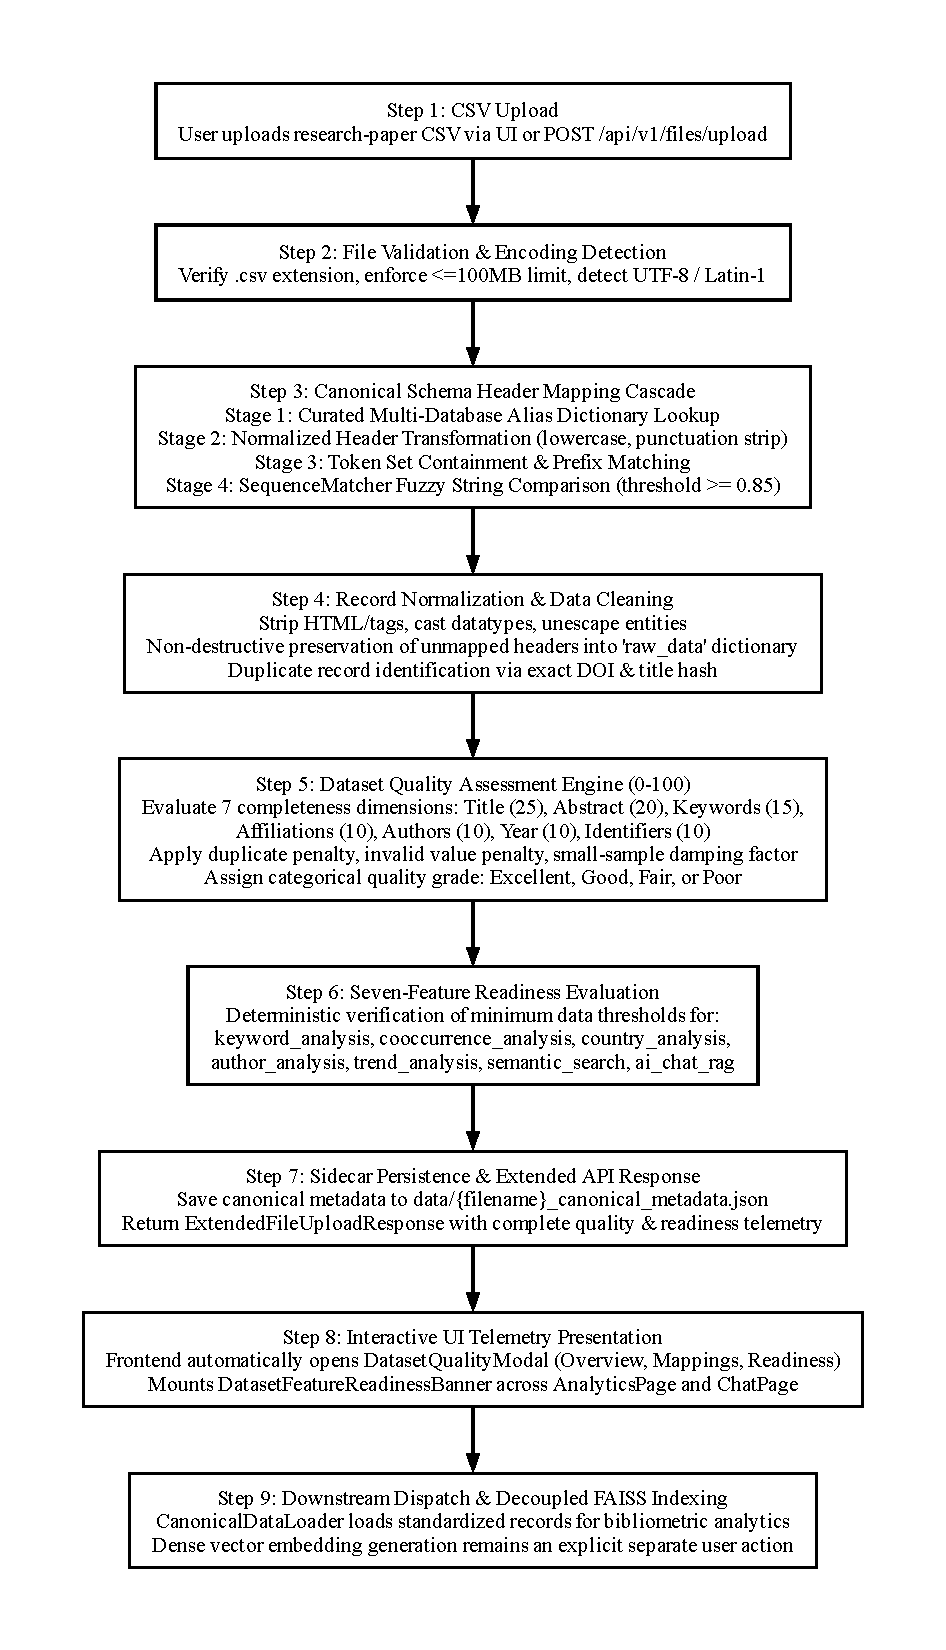
\includegraphics[width=0.92\textwidth]{figures/data_ingestion_workflow.pdf}
\caption{End-to-End Execution Sequence of the Universal Ingestion and Quality Engine}
\label{fig:data_ingestion_workflow}
\end{figure}

Figure~\ref{fig:data_ingestion_workflow} outlines the nine-stage ingestion pipeline executed whenever a user uploads an arbitrary research CSV file.

\subsection{Canonical Dataset Normalizer (dataset\_normalizer.py)}
The normalizer standardizes heterogeneous input schemas into a unified representation.

\subsubsection{The 20-Field Canonical Paper Schema}
The system maps all recognized data fields into a strict 20-field schema:
\begin{enumerate}
    \item \texttt{id}: Unique record identifier (derived from DOI, PMID, or deterministic row hash).
    \item \texttt{title}: Paper title string.
    \item \texttt{abstract}: Comprehensive manuscript abstract.
    \item \texttt{authors}: Delimited string or list of author names.
    \item \texttt{year}: 4-digit publication year (integer).
    \item \texttt{doi}: Digital Object Identifier normalized to standard format (e.g., \texttt{10.xxxx/...}).
    \item \texttt{pmid}: PubMed Unique Identifier.
    \item \texttt{pmcid}: PubMed Central Identifier.
    \item \texttt{journal}: Publishing journal or source venue name.
    \item \texttt{publisher}: Publishing organization.
    \item \texttt{keywords}: Author keywords or extracted key phrases.
    \item \texttt{mesh\_terms}: Medical Subject Headings (MeSH).
    \item \texttt{affiliations}: Author institutional affiliation strings.
    \item \texttt{countries}: Extracted sovereign country names.
    \item \texttt{citation\_count}: Inbound citation metric (integer).
    \item \texttt{reference\_count}: Outbound references count (integer).
    \item \texttt{url}: Primary landing page URL.
    \item \texttt{pdf\_url}: Direct PDF link.
    \item \texttt{source\_database}: Source repository identifier (e.g., \texttt{pubmed}, \texttt{scopus}).
    \item \texttt{raw\_data}: Dictionary preserving all original unmapped columns.
\end{enumerate}

\subsubsection{Four-Stage Header Matching Cascade}
To identify incoming columns without manual user mapping, the normalizer executes a four-tier matching cascade:
\begin{itemize}
    \item \textbf{Stage 1: Curated Alias Dictionary Lookup.} Matches headers against curated dictionaries containing hundreds of real-world aliases from major databases (e.g., matching \texttt{"Abstract (English)"}, \texttt{"AB"}, or \texttt{"Description"} to \texttt{abstract}).
    \item \textbf{Stage 2: Normalized Header Transformation.} Strips non-alphanumeric punctuation, converts text to lowercase, and evaluates canonical equivalence.
    \item \textbf{Stage 3: Token Set Containment.} Tokenizes multi-word headers and identifies canonical targets through token subset analysis.
    \item \textbf{Stage 4: Fuzzy String Matching.} Applies \texttt{difflib.SequenceMatcher} to detect typographical variants, assigning a mapping when string similarity $\ge 0.85$.
\end{itemize}

\subsubsection{Non-Destructive Raw Data Preservation}
No source information is ever discarded. Any column not mapped to the 20 canonical fields is automatically serialized into the \texttt{raw\_data} JSON dictionary for each record. The original uploaded CSV file is preserved intact on disk.

\subsection{Dataset Quality Assessment Engine (dataset\_quality.py)}
The quality engine evaluates dataset hygiene, computing an overall score between 0 and 100.

\subsubsection{Mathematical Quality Scoring Formula}
The base quality score represents a weighted summation of completeness across seven primary metadata dimensions:

\begin{equation}
\label{eq:quality_score}
\text{Base Score} = \sum_{i=1}^{7} W_i \times \text{Coverage}(A_i)
\end{equation}

\noindent where the weights $W_i$ are assigned as:
\begin{itemize}
    \item Title Coverage: 25\%
    \item Abstract Coverage: 20\%
    \item Keywords Coverage: 15\%
    \item Affiliations / Countries Coverage: 10\%
    \item Authors Coverage: 10\%
    \item Publication Year Coverage: 10\%
    \item Identifiers (DOI / PMID) Coverage: 10\%
\end{itemize}

\subsubsection{Deductions, Penalties, and Damping}
The final score applies deductions for duplicates and invalid values, scaled by a small-sample damping factor:

\begin{equation}
\text{Duplicate Penalty} = \min\left(10.0, \frac{\text{Duplicates}}{N} \times 20.0\right)
\end{equation}

\begin{equation}
\text{Invalid Penalty} = \min\left(5.0, \frac{\text{Invalids}}{N \times \text{Fields}} \times 25.0\right)
\end{equation}

\begin{equation}
\text{Damping Factor} = \min\left(1.0, \frac{N}{5.0}\right)
\end{equation}

\begin{equation}
\text{Final Quality Score} = \max\left(0.0, (\text{Base Score} - \text{Duplicate Penalty} - \text{Invalid Penalty}) \times \text{Damping Factor}\right)
\end{equation}

Datasets are categorized into quality grades: \textbf{Excellent} ($\ge 85$), \textbf{Good} ($\ge 70$), \textbf{Fair} ($\ge 50$), and \textbf{Poor} ($< 50$).

\subsection{Feature Readiness Assessment Engine}
Rather than allowing analytical jobs to crash at runtime due to missing data, the engine deterministically computes the operational readiness of all seven platform features.

\begin{figure}[H]
\centering
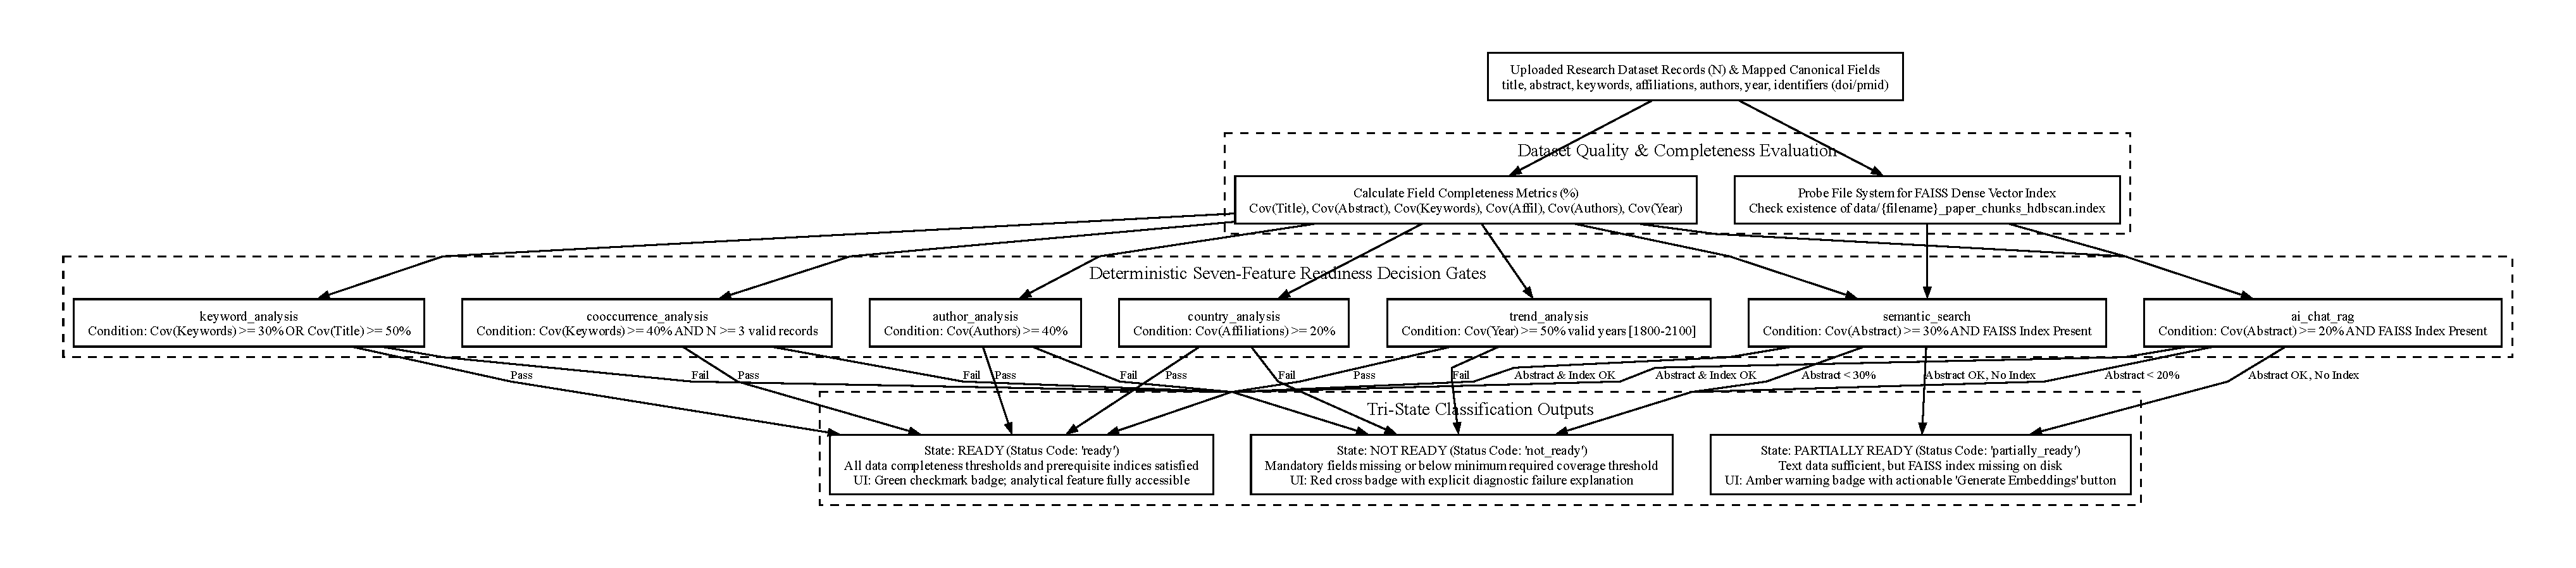
\includegraphics[width=0.92\textwidth]{figures/feature_readiness_workflow.pdf}
\caption{Deterministic Decision Logic of the Seven-Feature Readiness Evaluation Engine}
\label{fig:feature_readiness_workflow}
\end{figure}

As shown in Figure~\ref{fig:feature_readiness_workflow}, each feature is evaluated against specific data availability criteria and classified into one of three distinct operational states:
\begin{itemize}
    \item \textbf{Ready:} Mandatory fields meet or exceed completeness thresholds; feature is fully functional.
    \item \textbf{Partially Ready:} Primary data is available, but prerequisite secondary assets (such as FAISS vector indexes) have not yet been generated.
    \item \textbf{Not Ready:} Mandatory data fields are absent or fall below minimum viable thresholds.
\end{itemize}

Table~\ref{tab:feature_readiness_criteria} enumerates the verified decision criteria across all seven features.

\begin{table}[H]
\centering
\caption{Seven-Feature Readiness Decision Criteria and Thresholds}
\label{tab:feature_readiness_criteria}
\begin{tabularx}{\textwidth}{l X l}
\toprule
\textbf{Feature Identifier} & \textbf{Evaluation Criteria and Minimum Thresholds} & \textbf{Required Fields} \\
\midrule
\texttt{keyword\_analysis} & Keyword coverage $\ge 30\%$ OR Title coverage $\ge 50\%$ & \texttt{keywords}, \texttt{title} \\
\texttt{cooccurrence\_analysis} & Keyword coverage $\ge 40\%$ AND valid records $N \ge 3$ & \texttt{keywords} \\
\texttt{country\_analysis} & Affiliation or country coverage $\ge 20\%$ & \texttt{affiliations}, \texttt{countries} \\
\texttt{author\_analysis} & Author name coverage $\ge 40\%$ & \texttt{authors} \\
\texttt{trend\_analysis} & Valid publication year coverage $\ge 50\%$ (years 1800--2100) & \texttt{year} \\
\texttt{semantic\_search} & Abstract coverage $\ge 30\%$ AND FAISS index present on disk & \texttt{abstract}, FAISS index \\
\texttt{ai\_chat\_rag} & Abstract coverage $\ge 20\%$ AND FAISS index present on disk & \texttt{abstract}, FAISS index \\
\bottomrule
\end{tabularx}
\end{table}

\subsection{Canonical Data Loader (canonical\_loader.py)}
The \texttt{CanonicalDataLoader} class serves as the unified programmatic interface for consuming normalized records. When analytical services invoke:

\begin{lstlisting}[language=python]
df, metadata = CanonicalDataLoader.load_canonical_dataframe(
    filename="uploaded_paper.csv",
    exclude_duplicates=True
)
\end{lstlisting}

\noindent the loader checks for an existing sidecar cache (\texttt{data/uploaded\_paper\_canonical\_metadata.json}). If present, it loads the cached telemetry; if absent, it executes on-the-fly normalization, creates the sidecar cache, and returns a clean, deduplicated Pandas DataFrame. Furthermore, \texttt{apply\_index\_status\_overlay()} dynamically checks disk storage for vector indexes, ensuring that readiness telemetry always reflects real-time file availability.

\subsection{Frontend Telemetry Integration}
The frontend presents this telemetry through two primary components:
\begin{itemize}
    \item \textbf{Dataset Quality Modal (\texttt{DatasetQualityModal.tsx}):} Automatically opens upon CSV upload. Contains three interactive tabs: \textit{Overview} (Overall Score, Grade, Hygiene Metrics), \textit{Column Mappings} (Mapped vs Unmapped Columns, Recognition Confidence), and \textit{Feature Readiness} (Tri-state badges and diagnostic guidance).
    \item \textbf{Dataset Feature Readiness Banner (\texttt{DatasetFeatureReadinessBanner.tsx}):} Persistently mounted at the top of \texttt{AnalyticsPage.tsx} and \texttt{ChatPage.tsx}. Alerts researchers if analytical features are limited by dataset quality or missing embeddings.
\end{itemize}

\noindent \textbf{Decoupled Embedding Architecture:} Uploading a CSV file does \textbf{not} automatically generate dense vector embeddings. Generating embeddings remains an explicit, user-initiated operation via the UI or API. If a dataset has sufficient abstracts but lacks a FAISS index, \texttt{semantic\_search} and \texttt{ai\_chat\_rag} are reported as \textbf{Partially Ready} with an actionable prompt to generate embeddings.

\newpage
\section{API Reference and Route Specifications}
\label{sec:api_reference}

\subsection{REST API Design Principles}
Research Rover's backend exposes a standardized RESTful API rooted at \texttt{/api/v1}. All responses return JSON payloads with standard HTTP status codes ($200$ OK, $400$ Bad Request, $404$ Not Found, $500$ Internal Server Error).

\subsection{Complete Route Inventory}
Table~\ref{tab:api_route_inventory} provides an exhaustive inventory of the verified FastAPI endpoints implemented across the platform.

\begin{longtable}{l p{5.5cm} p{2.2cm} X}
\caption{Comprehensive FastAPI REST Route Specifications} \label{tab:api_route_inventory} \\
\toprule
\textbf{HTTP Method} & \textbf{Endpoint Path} & \textbf{Router} & \textbf{Functional Purpose} \\
\midrule
\endfirsthead
\toprule
\textbf{HTTP Method} & \textbf{Endpoint Path} & \textbf{Router} & \textbf{Functional Purpose} \\
\midrule
\endhead
\bottomrule
\endfoot
\texttt{GET} & \texttt{/} & Core & Lightweight API health ping \\
\texttt{GET} & \texttt{/health} & Core & Detailed runtime status and model health \\
\texttt{GET} & \texttt{/api/v1/system/status} & System & Reports runtime memory and loaded AI models \\
\midrule
\texttt{POST} & \texttt{/api/v1/search/} & Search & Initiates PubMed/OpenAlex literature search \\
\texttt{GET} & \texttt{/api/v1/search/progress} & Search & Streams search execution progress via SSE \\
\texttt{POST} & \texttt{/api/v1/search/cancel} & Search & Cancels an active background search job \\
\texttt{GET} & \texttt{/api/v1/search/results} & Search & Retrieves paginated search results \\
\midrule
\texttt{POST} & \texttt{/api/v1/files/upload} & Files & Ingests, normalizes, and scores uploaded CSV \\
\texttt{GET} & \texttt{/api/v1/files/\{filename\}/quality} & Files & Returns quality score and readiness telemetry \\
\texttt{GET} & \texttt{/api/v1/files/list} & Files & Lists all available research CSV datasets \\
\texttt{GET} & \texttt{/api/v1/files/download/\{filename\}} & Files & Downloads raw or analyzed CSV file \\
\texttt{GET} & \texttt{/api/v1/files/csv/\{filename\}/data} & Files & Returns complete raw CSV tabular data \\
\texttt{GET} & \texttt{/api/v1/files/csv/\{filename\}/paginated} & Files & Returns paginated dataset rows with sorting \\
\texttt{DELETE} & \texttt{/api/v1/files/\{filename\}} & Files & Deletes dataset, sidecars, and vector indexes \\
\texttt{GET} & \texttt{/api/v1/files/download-pdf} & Files & Downloads paper full-text PDF if accessible \\
\midrule
\texttt{POST} & \texttt{/api/v1/analysis/generate} & Analysis & Triggers bibliometric frequency analysis \\
\texttt{GET} & \texttt{/api/v1/analysis/\{filename\}/summary} & Analysis & Returns keyword counts and summary metrics \\
\texttt{GET} & \texttt{/api/v1/analysis/\{filename\}/matrix} & Analysis & Returns keyword co-occurrence matrix \\
\texttt{GET} & \texttt{/api/v1/analysis/\{filename\}/countries} & Analysis & Returns sovereign country collaboration counts \\
\texttt{GET} & \texttt{/api/v1/analysis/\{filename\}/country-collaboration} & Analysis & Returns 2D/3D collaboration graph topology \\
\texttt{POST} & \texttt{/api/v1/analysis/\{filename\}/regenerate} & Analysis & Forces recalculation of bibliometric data \\
\midrule
\texttt{POST} & \texttt{/api/v1/embeddings/\{filename\}} & Embeddings & Generates dense embeddings and FAISS index \\
\texttt{GET} & \texttt{/api/v1/embeddings/progress} & Embeddings & Returns real-time embedding progress \\
\texttt{POST} & \texttt{/api/v1/embeddings/cancel} & Embeddings & Cancels active vector embedding generation \\
\texttt{GET} & \texttt{/api/v1/embeddings/\{filename\}/status} & Embeddings & Checks whether FAISS index exists on disk \\
\texttt{DELETE} & \texttt{/api/v1/embeddings/\{filename\}} & Embeddings & Deletes FAISS index and chunk mappings \\
\midrule
\texttt{POST} & \texttt{/api/v1/chat/} & Chat & Dispatches RAG conversational query across papers \\
\texttt{POST} & \texttt{/api/v1/chat/\{filename\}} & Chat & Dispatches RAG query scoped to a single dataset \\
\end{longtable}

\subsection{Key Endpoint Payloads and Responses}

\subsubsection{Dataset Upload Endpoint: POST /api/v1/files/upload}
\textbf{Request:} \texttt{multipart/form-data} containing \texttt{file: UploadFile}.\\
\textbf{Response Schema (\texttt{ExtendedFileUploadResponse}):}
\begin{lstlisting}[language=json]
{
  "filename": "machine_learning_cancer.csv",
  "message": "File uploaded and processed successfully",
  "total_records": 150,
  "valid_records": 148,
  "duplicate_records": 2,
  "quality_score": 87.5,
  "quality_grade": "Excellent",
  "field_mappings": {
    "Title": "title",
    "Abstract Text": "abstract",
    "Author Names": "authors",
    "PubYear": "year"
  },
  "unmapped_columns": ["Scopus_Internal_ID"],
  "feature_readiness": {
    "keyword_analysis": {"status": "ready", "warnings": []},
    "semantic_search": {
      "status": "partially_ready",
      "warnings": ["FAISS vector index missing. Generate embeddings to enable."]
    }
  }
}
\end{lstlisting}

\subsubsection{Quality Telemetry Endpoint: GET /api/v1/files/\{filename\}/quality}
\textbf{Path Parameter:} \texttt{filename} (string, name of CSV dataset).\\
\textbf{Response Schema (\texttt{DatasetQualityReport}):} Returns the cached or computed quality score, field completeness percentages, penalty deductions, and feature readiness telemetry.

\newpage
\section{Troubleshooting and Diagnostic Procedures}
\label{sec:troubleshooting}

This section details practical diagnostic workflows and verified technical solutions for common configuration, installation, and runtime issues.

\subsection{Python Virtual Environment and Execution Policy Errors}
\textbf{Symptom:} Windows PowerShell displays \texttt{File .venv\textbackslash Scripts\textbackslash Activate.ps1 cannot be loaded because running scripts is disabled on this system.}\\
\textbf{Root Cause:} Windows PowerShell execution policy restricts execution of unsigned local scripts by default.\\
\textbf{Solution:} Open PowerShell as CurrentUser and enable script execution:
\begin{lstlisting}[language=powershell]
Set-ExecutionPolicy -ExecutionPolicy RemoteSigned -Scope CurrentUser
\end{lstlisting}

\subsection{Dependency Installation and Wheel Compilation Failures}
\textbf{Symptom:} \texttt{pip install -r requirements.txt} fails while compiling \texttt{faiss-cpu}, \texttt{hdbscan}, or \texttt{Crawl4AI} with \texttt{Microsoft Visual C++ 14.0 or greater is required.}\\
\textbf{Root Cause:} The host machine lacks pre-built binary wheels for the local Python version, prompting \texttt{pip} to build from C++ source.\\
\textbf{Solution:} 
\begin{enumerate}
    \item Verify that Python 3.11.x 64-bit is being used. Pre-compiled wheels exist on PyPI for 64-bit Python 3.11 on Windows, macOS, and Linux.
    \item Upgrade packaging utilities: \texttt{python -m pip install --upgrade pip setuptools wheel}.
    \item If compiling from source is necessary, install the \textit{Visual Studio C++ Build Tools} from Microsoft.
\end{enumerate}

\subsection{Port Collisions and Binding Failures}
\textbf{Symptom:} Uvicorn fails to start with \texttt{ERROR: [Errno 10048] error while attempting to bind on address ('0.0.0.0', 8000): only one usage of each socket address is normally permitted.}\\
\textbf{Root Cause:} A previous instance of Uvicorn or another local application is occupying TCP port 8000.\\
\textbf{Solution:} Identify and terminate the occupying process in PowerShell:
\begin{lstlisting}[language=powershell]
# Locate process ID (PID) occupying port 8000
Get-NetTCPConnection -LocalPort 8000 | Select-Object OwningProcess

# Terminate process by PID (e.g., PID 14220)
Stop-Process -Id 14220 -Force
\end{lstlisting}
\noindent Repeat for port 3000 if the Vite development server reports a port collision.

\subsection{Frontend API Proxy and CORS Connectivity Issues}
\textbf{Symptom:} Frontend UI reports \texttt{Network Error} or browser console displays \texttt{ERR\_CONNECTION\_REFUSED} when searching or uploading datasets.\\
\textbf{Root Cause:} The FastAPI backend server is not running on port 8000, or the Vite proxy is misconfigured.\\
\textbf{Solution:}
\begin{enumerate}
    \item Confirm that Uvicorn is active in Terminal 1 and responds to \url{http://localhost:8000/health}.
    \item Verify that \texttt{frontend/vite.config.ts} contains the active proxy block forwarding \texttt{/api} to \texttt{http://localhost:8000}.
    \item If accessing across a local area network, configure \texttt{VITE\_API\_BASE_URL} explicitly in \texttt{frontend/.env}.
\end{enumerate}

\subsection{Missing API Key or Authentication Failures}
\textbf{Symptom:} Chat queries return \texttt{500 Internal Server Error} with backend logs displaying \texttt{GoogleGenerativeAIError: API key not valid.}\\
\textbf{Root Cause:} The \texttt{GOOGLE\_GENAI\_API\_KEY} variable in \texttt{backend/.env} is blank or invalid.\\
\textbf{Solution:}
\begin{enumerate}
    \item Visit Google AI Studio (\url{https://aistudio.google.com/apikey}) and generate a valid API key.
    \item Open \texttt{backend/.env} and ensure the key is placed without quotation errors:
    \begin{lstlisting}
    GOOGLE_GENAI_API_KEY="AIzaSyYourKeyHere"
    \end{lstlisting}
    \item Restart Uvicorn to ensure environment variables are reloaded.
\end{enumerate}

\subsection{FAISS Missing-Index Warning (Partially Ready Status)}
\textbf{Symptom:} The Dataset Quality Modal displays an amber warning stating \texttt{FAISS vector index missing} and classifies Semantic Search as \textit{Partially Ready}.\\
\textbf{Root Cause:} By design, Research Rover decouples dataset upload from computationally heavy vector embedding generation.\\
\textbf{Solution:} This is normal behavior, not a system defect. In the UI, click \textbf{Generate Embeddings} (or issue \texttt{POST /api/v1/embeddings/\{filename\}}). Once the Sentence Transformer finishes encoding, the status automatically transitions to \textbf{Ready}.

\subsection{CSV Encoding and Parsing Problems}
\textbf{Symptom:} Dataset upload fails with \texttt{UnicodeDecodeError: 'utf-8' codec can't decode byte...}\\
\textbf{Root Cause:} The uploaded CSV file was exported using Windows-1252, ISO-8859-1 (Latin-1), or UTF-16 with a Byte Order Mark (BOM).\\
\textbf{Solution:} Research Rover's \texttt{dataset\_normalizer.py} automatically attempts Latin-1 decoding if UTF-8 fails. If a corrupted file persists, open the CSV in Microsoft Excel or VS Code and re-save using \textbf{CSV UTF-8 (Comma delimited) (*.csv)}.

\newpage
\section{Project Directory Structure}
\label{sec:directory_structure}

\subsection{Repository Layout}
The Research Rover repository follows a modular software engineering structure designed for maintainability and scalability. Below is an annotated hierarchy of essential directories and files:

\begin{lstlisting}[caption={Annotated Research Rover Project Tree}]
Research_Rover/
├── README.md                      # Primary project overview and instructions
├── .gitignore                     # Git exclusion rules (.venv, data, node_modules)
│
├── backend/                       # Python 3.11+ / FastAPI Application
│   ├── main.py                    # Application entry point, lifespan, CORS, routes
│   ├── requirements.txt           # Pinned production and research dependencies
│   ├── .env.example               # Reference environment variable configuration
│   ├── .env                       # Local secrets (API keys - excluded from Git)
│   │
│   ├── app/
│   │   ├── api/
│   │   │   └── routes/            # REST API Router Controllers
│   │   │       ├── analysis.py    # Keyword and country analytics endpoints
│   │   │       ├── chat.py        # Gemini conversational RAG endpoints
│   │   │       ├── embeddings.py  # FAISS dense vector indexing endpoints
│   │   │       ├── files.py       # Dataset upload, quality, download endpoints
│   │   │       ├── search.py      # PubMed/OpenAlex search & progress endpoints
│   │   │       └── system.py      # Runtime model status and health endpoints
│   │   │
│   │   ├── core/                  # Core Application Infrastructure
│   │   │   ├── config.py          # Pydantic BaseSettings and env file loader
│   │   │   ├── dependencies.py    # FastAPI dependency injection providers
│   │   │   ├── logging.py         # Standardized application logging setup
│   │   │   └── model_manager.py   # Asynchronous transformer model lifecycle manager
│   │   │
│   │   ├── models/
│   │   │   └── schemas.py         # Pydantic request/response data contracts
│   │   │
│   │   ├── services/              # Core Domain Business Logic
│   │   │   ├── analysis_service.py       # Keyword frequencies & co-occurrence
│   │   │   ├── canonical_loader.py       # Unified data loader & sidecar caching
│   │   │   ├── chat_service.py           # Gemini RAG query decomposition
│   │   │   ├── country_service.py        # International collaboration graphs
│   │   │   ├── dataset_normalizer.py     # 20-field canonical normalization
│   │   │   ├── dataset_quality.py        # Quality scoring & 7-feature readiness
│   │   │   ├── embedding_service.py      # Sentence Transformers & FAISS logic
│   │   │   ├── openalex_service.py       # OpenAlex scholarly API integration
│   │   │   ├── pubmed_service.py         # NCBI E-utilities search integration
│   │   │   ├── reranker_service.py       # MedCPT bi-encoder neural re-ranking
│   │   │   └── unified_search_service.py # Multi-source search & deduplication
│   │   │
│   │   └── utils/
│   │       ├── country_extractor.py      # Affiliation regex country parser
│   │       └── csv_loader.py             # Basic CSV reading helpers
│   │
│   ├── features/
│   │   └── embedding_and_indexing.py     # Chunking and vector indexing scripts
│   │
│   └── tests/                     # Automated Test Suites (57 Verified Tests)
│       ├── test_dataset_normalizer.py    # 18 Normalizer unit tests
│       ├── test_dataset_quality.py       # 10 Quality engine unit tests
│       └── test_dataset_integration.py   # 29 API integration tests
│
├── frontend/                      # React 19 / TypeScript / Vite Application
│   ├── package.json               # Node.js dependencies and run scripts
│   ├── vite.config.ts             # Vite dev server port 3000 & API reverse proxy
│   ├── tsconfig.json              # TypeScript compilation rules
│   │
│   └── src/
│       ├── components/            # Reusable UI & Telemetry Components
│       │   ├── CountryAnalysisView.tsx            # Country graphs orchestrator
│       │   ├── CountryCollaboration2D.tsx         # 2D ForceGraph canvas
│       │   ├── CountryCollaboration3D.tsx         # Three.js 3D ForceGraph sphere
│       │   ├── DatasetFeatureReadinessBanner.tsx  # Persistent readiness banner
│       │   ├── DatasetQualityModal.tsx            # Multi-tab quality modal
│       │   ├── EmbeddingProgressModal.tsx         # FAISS indexing progress modal
│       │   └── WorldMap.tsx                       # Mercator world map projection
│       │
│       ├── pages/                 # Full Application View Pages
│       │   ├── AnalyticsPage.tsx  # Bibliometric analytics dashboard
│       │   ├── ChatPage.tsx       # Conversational AI RAG research assistant
│       │   ├── HomePage.tsx       # Welcome and platform overview page
│       │   ├── SearchPage.tsx     # Literature discovery and query portal
│       │   └── UseCasesPage.tsx   # Verified academic workflows demonstration
│       │
│       ├── services/
│       │   └── api.ts             # Axios HTTP client, types, and API calls
│       │
│       └── types/
│           └── index.ts           # Shared TypeScript interfaces and contracts
│
└── data/                          # Runtime Storage Layer (Generated at Startup)
    ├── *.csv                      # Downloaded and uploaded research datasets
    ├── *_canonical_metadata.json  # Ingestion quality & readiness sidecars
    ├── *_paper_chunks_hdbscan.index # FAISS dense vector binary indexes
    └── *_full_text_mapping.json   # Scraped DOI-to-text mapping files
\end{lstlisting}

\newpage
\section{Conclusion and Future Work}
\label{sec:conclusion}

\subsection{Summary of Technical Contribution}
This documentation has presented the complete architectural, deployment, and operational specification for \textbf{Research Rover}. By uniting multi-source literature retrieval (PubMed and OpenAlex), neural semantic re-ranking (MedCPT), dense vector indexing (Sentence Transformers and FAISS), and retrieval-augmented conversational generation (Google Gemini), Research Rover offers a comprehensive environment for data-driven scientific inquiry.

The development and integration of the \textbf{Universal Dataset Ingestion and Quality Analysis System} represents a transformative enhancement to the platform's reliability. By introducing:
\begin{enumerate}
    \item A resilient \textbf{20-field canonical schema} with a four-tier header matching cascade,
    \item Multi-attribute \textbf{quality scoring} (0--100) with duplicate and invalid value deductions,
    \item Deterministic \textbf{seven-feature readiness evaluation} guarding downstream analytics, and
    \item Transparent \textbf{frontend telemetry integration} via modals and banners,
\end{enumerate}
Research Rover effectively eliminates brittle column dependencies, shields bibliometric algorithms from corrupt inputs, and provides researchers with complete clarity regarding dataset hygiene before initiating computational workflows.

\subsection{Directions for Future Extension}
Subsequent engineering iterations may explore the following extensions:
\begin{itemize}
    \item \textbf{Interactive Header Remapping:} Expanding the frontend Dataset Quality Modal to allow researchers to manually correct or assign unmapped columns and persist those overrides into the sidecar.
    \item \textbf{Expanded File Formats:} Extending the ingestion pipeline beyond delimited CSV files to natively parse BibTeX (\texttt{.bib}), Research Information Systems (\texttt{.ris}), and EndNote XML formats.
    \item \textbf{Automated Index Synchronization:} Incorporating cryptographic hash validation between stored FAISS vector indexes and parent CSV datasets to automatically flag stale embeddings when records are appended.
    \item \textbf{Distributed Vector Stores:} Transitioning FAISS CPU indexes to distributed vector databases (e.g., Milvus or Qdrant) for multi-million document enterprise scaling.
\end{itemize}


% ---------------------------------------------------------------------------
% BIBLIOGRAPHY
% ---------------------------------------------------------------------------
\newpage
\bibliographystyle{plain}
\bibliography{references}

\end{document}